\documentclass[letterpaper,12pt]{article}
\usepackage{array}
\usepackage{threeparttable}
\usepackage{geometry}
\geometry{letterpaper,tmargin=1in,bmargin=1in,lmargin=1.25in,rmargin=1.25in}
\usepackage{fancyhdr,lastpage}
\pagestyle{fancy}
\lhead{}
\chead{}
\rhead{}
\lfoot{}
\cfoot{}
\rfoot{\footnotesize\textsl{Page \thepage\ of \pageref{LastPage}}}
\renewcommand\headrulewidth{0pt}
\renewcommand\footrulewidth{0pt}
\usepackage[format=hang,font=normalsize,labelfont=bf]{caption}
\usepackage{listings}
\lstset{frame=single,
  language=Python,
  showstringspaces=false,
  columns=flexible,
  basicstyle={\small\ttfamily},
  numbers=none,
  breaklines=true,
  breakatwhitespace=true
  tabsize=3
}
\usepackage{amsmath}
\usepackage{amssymb}
\usepackage{amsthm}
\usepackage{harvard}
\usepackage{setspace}
\usepackage{breqn}
\usepackage{float,color}
\usepackage[pdftex]{graphicx}
\usepackage{hyperref}
\hypersetup{colorlinks,linkcolor=red,urlcolor=blue}
\theoremstyle{definition}
\newtheorem{theorem}{Theorem}
\newtheorem{acknowledgement}[theorem]{Acknowledgement}
\newtheorem{algorithm}[theorem]{Algorithm}
\newtheorem{axiom}[theorem]{Axiom}
\newtheorem{case}[theorem]{Case}
\newtheorem{claim}[theorem]{Claim}
\newtheorem{conclusion}[theorem]{Conclusion}

\newtheorem{conjecture}[theorem]{Conjecture}
\newtheorem{corollary}[theorem]{Corollary}
\newtheorem{criterion}[theorem]{Criterion}
\newtheorem{definition}[theorem]{Definition}
\newtheorem{derivation}{Derivation} % Number derivations on their own
\newtheorem{example}[theorem]{Example}
\newtheorem{exercise}[theorem]{Exercise}
\newtheorem{lemma}[theorem]{Lemma}
\newtheorem{notation}[theorem]{Notation}
\newtheorem{problem}[theorem]{Problem}
\newtheorem{proposition}{Proposition} % Number propositions on their own
\newtheorem{remark}[theorem]{Remark}
\newtheorem{solution}[theorem]{Solution}
\newtheorem{summary}[theorem]{Summary}
%\numberwithin{equation}{section}
\bibliographystyle{aer}
\newcommand\ve{\varepsilon}
\newcommand\boldline{\arrayrulewidth{1pt}\hline}
\renewcommand{\vec}[1]{\mathbf{#1}}
%\newcommand\norm[1]{\left\lVert#1\right\rVert}


\begin{document}

\begin{flushleft}
  \textbf{\large{Problem Set \#5}} \\
  Smooth and convex optimization \\
  Shirley Yuan, collaborated with Winston, Fiona and Zeshun
\end{flushleft}


\noindent\textbf{Exercise 8.1}\\
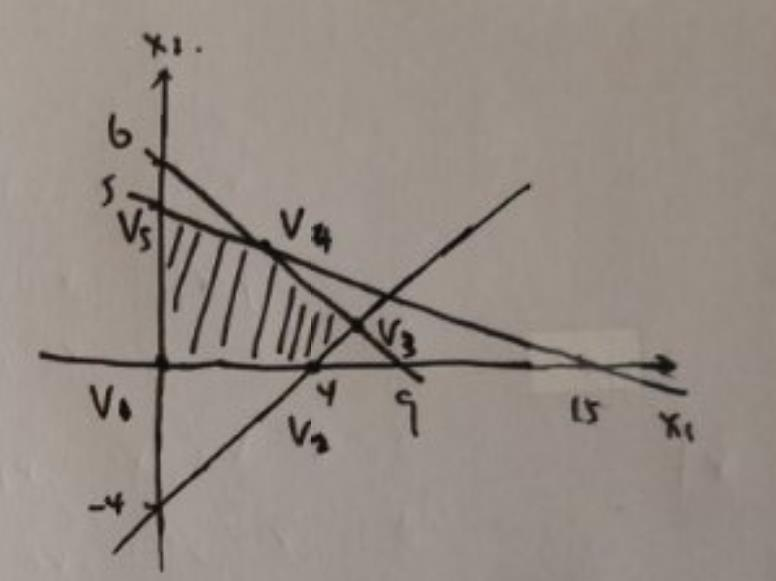
\includegraphics{11.png}\\

The feasible set is shown above. Observe that there are five vertices. $V_1 = (0,0), V_2 = (1,0), V_3 = (\frac{37}{7}, \frac{5}{7}), V_4 = (\frac{16}{5}, \frac{14}{5}), V_5 = (1,0).$ Easy calculation yields that $(\frac{37}{7}, \frac{5}{7})$ is an optimizer, and the optimized value is $\frac{165}{7}.$ \\



\noindent\textbf{Exercise 8.2} \\
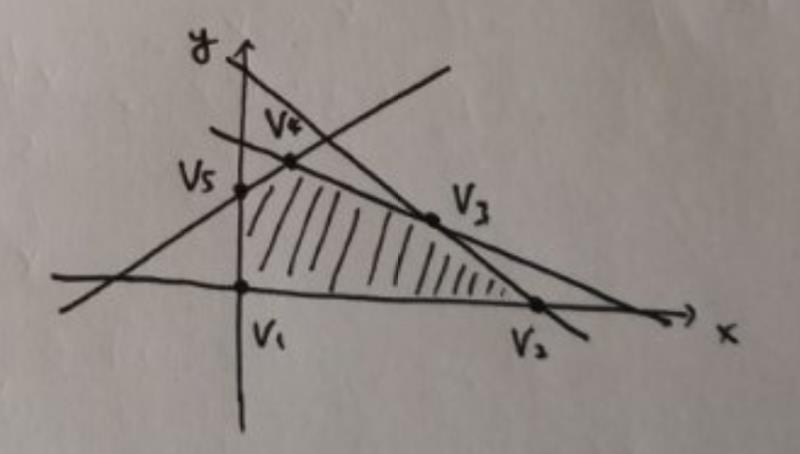
\includegraphics{12.png}\\
(1) The feasible set is shown above. Observe that there are five vertices. $V_1 = (0,0), V_2 = (4,0), V_3 = (6, 2), V_4 = (3, 4), V_5 = (5,0).$ Easy calculation yields that $(6, 2)$ is an optimizer, and the optimized value is $20.$ \\
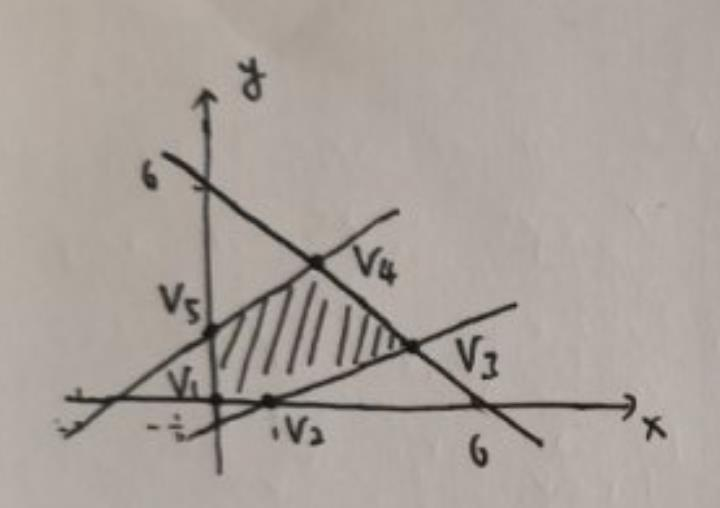
\includegraphics{13.png}\\
(2) The feasible set is shown above. Observe that there are five vertices. $V_1 = (0,0), V_2 = (27,0), V_3 = (15, 12), V_4 = (5, 16), V_5 = (11,0).$ Easy calculation yields that $(15, 12)$ is an optimizer, and the optimized value is $132.$ \\

\noindent\textbf{Exercise 8.3} \\
\begin{align*}
  \max &\{4x + 3y\} \\
  \text{subject to } &15x+10y \leq 1800 \\
  &2x+2y \leq 300 \\
  &y\leq 200 \\
  &x, y \geq 0.
\end{align*}

\noindent\textbf{Exercise 8.4} \\
\begin{align*}
  \max &\{2x_{AB} + 5x_{BC} + 2x_{CF} + 5x_{AD} + 2x_{BD} + 7x_{BE} + 9x_{BF} + 4x_{DE} +3x_{EF}\} \\
  \text{subject to } &x_{AD} + x_{AB} = 10 \\
  &x_{BC} + x_{BE} - x_{AB} = 1 \\
  &x_{CF} - x_{BC} = -2 \\
  &x_{DE} - x_{AD} - x_{BD} = -3 \\
  &x_{EF} - x_{BE} - x_{DE} = 4 \\
  &-x_{CF} - x_{EF} - x_{BF} = -10 \\
  &0\leq x_{AB} \leq 6 \\
  &0\leq x_{BC} \leq 6 \\
  &0\leq x_{CF} \leq 6 \\
  &0\leq x_{AD} \leq 6 \\
  &0\leq x_{BD} \leq 6 \\
  &0\leq x_{BE} \leq 6 \\
  &0\leq x_{BF} \leq 6 \\
  &0\leq x_{DE} \leq 6 \\
  &0\leq x_{EF} \leq 6.
\end{align*}

\noindent\textbf{Exercise 8.5} \\
(1)

\begin{align*}
  \xi &= 3x_1 + x_2 \\
  w_1 &= 15 - x_1 - 3x_2\\
  w_2 &= 18 - 2x_1 - 3x_2 \\
  w_3 &= 4 - x_1 + x_2
\end{align*}

Observe that we can increase $x_1$ to $9.$
\begin{align*}
  \xi &= 12 + 4x_2 - 3w_3 \\
  w_1 &= 11 - 3x_2 - w_3  \\
  w_2 &= 10 - 5x_2 + 2w_3 \\
  x_1 &= 4 + x_2 - w_3
\end{align*}
Observe that we can increase $x_2$ to $2.$
\begin{align*}
  \xi &= 20 - 0.8w_2 - 1.4w_3 \\
  w_1 &= 5 + 0.6 w_2 - 2.2 w_3 \\
  x_2 &= 2 - 0.2w_2 + 0.4w_3 \\
  x_1 &= 6 + 0.2w_2 - 0.6w_3
\end{align*}
There is no more term to increase and we conclude that the optimal value is $20$ when $x_1 = 6, x_2 =2.$

(2)
\begin{align*}
  \xi &= 4x+6y \\
  w_1 &= 27 -x-y \\
  w_2 &= 27-x-y \\
  w_3 &= 90-2x-5y
\end{align*}
Observe that we can increase $x \text{ to } 27.$
\begin{align*}
  \xi &= 108 - 4w_2 +2y \\
  w_1 &= 38 - w_2 - 2y \\
  x &= 27 - w_2 - y \\
  w_3 &= 36 + 2w_2 - 3y
\end{align*}
Observe that we can increase $y \text{ to } 12.$
\begin{align*}
  \xi &= 132 - \frac{8}{3}w_2 + \frac{2}{3} w_3\\
  w_1 &= 38 - \frac{7}{3}w_2 - \frac{2}{3}w_3 \\
  x &= 15 - \frac{5}{3}w_2 - \frac{1}{3}w_3 \\
  y &= 12 + \frac{2}{3}w_2 + \frac{1}{3}w_3
\end{align*}
There is no more term to increase and we conclude that the optimal value is $132$ when $x = 15, y =12.$ \\

\noindent\textbf{Exercise 8.6} \\
Observe that our problem
\begin{align*}
  \max &\{4x + 3y\} \\
  \text{subject to } &15x+10y \leq 1800 \\
  &2x+2y \leq 300 \\
  &y\leq 200 \\
  &x, y \geq 0
\end{align*}
is equivalent to
\begin{align*}
  \max &\{4x + 3y\} \\
  \text{subject to } &3x+2y \leq 360 \\
  &x+y \leq 150 \\
  &y\leq 200 \\
  &x, y \geq 0.
\end{align*} \\
\begin{align*}
  \xi &= 4x+3y \\
  w_1 &= 360 -3x-2y \\
  w_2 &= 150 -x-y \\
  w_3 &= 200 -7
\end{align*}
Observe that we can increase $y \text{ to } 150.$
\begin{align*}
  \xi &= 450 + x - 3w_2 \\
  w_1 &= 60 -x +2w_2 \\
  y &= 150 -x -w_2 \\
  w_3 &= 50 + x + w_2
\end{align*}
Observe that we can increase $x \text{ to } 60.$
\begin{align*}
  \xi &= 510 - w_1 - w_2 \\
  x &= 60 - w_1 + 2 w_2 \\
  y &= 90 + w_1 - 3w_2 \\
  w_3 &= 110 - w_1 + 3w_2
\end{align*}
There is no more term to increase and we conclude that the optimal value is $510$ when $x = 60, y =90.$ So the company should produce 60 toy soldiers and 90 toy dolls. \\

\noindent\textbf{Exercise 8.7} \\
(1) Observe that the origin is not in the feasible set, so we need an auxillary problem to find an inital vertex, which is
\begin{align*}
  \max &\{ -x_0\} \\
  \text{subject to } & -4x_1 -2x_2 -x_0 \leq -8 \\
  &-2x_1 + 3x_2 -x_0 \leq 6\\
  &x_1 + x_0 \leq 3 \\
  &x_0, x_1, x_2 \geq 0
\end{align*}
We use simplex method to solve it:
\begin{align*}
  \xi &= -x_0 \\
  w_1 &= -8+4x_1 +2x_2 +x_0 \\
  w_2 &= 6 + 2x_1 - 3x_2 + x_0 \\
  w_3 &= 3 - x_1 - x_0
\end{align*}
We start with $x_0 = 8.$
\begin{align*}
  \xi &= -8 - w_1 + 4x_1 + 2x_2 \\
  x_0 &= 8 + w_1 -4x_1 - 2x_2 \\
  w_2 &= 14 + w_1 - 2x_1 - 5x_2 \\
  w_3 &= -5 - w_1 + 3x_1 + 2x_2
\end{align*}
Observe that we can increase $x_1 \text{ to } 2.$
\begin{align*}
  \xi &= -x_0 \\
  x_1 &= 2 + 0.25 w_1 - 0.5 x_2 - 0.25 x_0 \\
  w_2 &= 10 + 0.5w_1 + x_2 + 0.5x_0\\
  w_3 &= 1 - 0.25 w_1 + 0.5x_2 -0.75x_0
\end{align*}
Hence we can see that a feasible vertex is $x_1 = 2, x_2 = 0.$ We start from the original problem and let $x_1$ be $2$.
\begin{align*}
  \xi &= 2 + 1.5x_2 + 0.5 w_1\\
  x_1 &= 2 - 0.5x_2 + 0.5w_1 \\
  w_2 &= 10 + w_1 - 4x_2 \\
  w_3 &= 1 + 0.5 x_2 - 0.5w_1
\end{align*}
Observe that we can incrase $w_1$ to $2.$
\begin{align*}
  \xi &= 3 + 2 x_2 - w_3 \\
  x_1 &= 3 - w_3 \\
  w_2 &= 12 - 3x_2 - 2w_3 \\
  w_1 &= 2 + x_2 -2w_3
\end{align*}
Observe that we can incrase $x_2$ to $4.$
\begin{align*}
  \xi &= 11 - \frac{2}{3}w_2 - \frac{7}{3}w_3 \\
  x_1 &= 3 - w_3 \\
  x_2 &= 4 - \frac{1}{3}w_2 -\frac{2}{3}w_3 \\
  w_1 &= 6 - \frac{1}{3}w_2 -\frac{8}{3}w_3
\end{align*}
There is no more term to increase. So the optimal value is $11$ when $x_1 =3, x_2 = 4.$ \\
(2)Write down the auxillary problem and we can see that $x_0$ can never be $0.$ So this problem is infeasible.  \\
(3)We write down the table.
\begin{align*}
  \xi &= -3x_1 + x_2 \\
  w_1 &= 4 - x_2 \\
  w_2 &= 6+2x_1 -3x_2 \\
\end{align*}
Observe that we can increase $x_2$ to $2.$
\begin{align*}
  \xi &= 2 - \frac{7}{3}x_1 - \frac{1}{3}w_2 \\
  w_1 &= 2 - \frac{2}{3}x_1 + \frac{1}{3}w_2 \\
  x_2 &= 2 + \frac{2}{3}x_1 \frac{1}{3}w_2
\end{align*}
There is no more term to increase. So the optimal value is $2$ when $x_1 =0, x_2 = 2.$ \\


\noindent\textbf{Exercise 8.8} \\
$$\max{-x_1-x_2-x_3} \text{ s.t. } x_1, x_2, x_3 \geq 0.$$
\noindent\textbf{Exercise 8.9} \\
$$\max{x_1+x_2+x_3} \text{ s.t. } x_1, x_2, x_3 \geq 0.$$
\noindent\textbf{Exercise 8.10} \\
$$\max{x_1+x_2+x_3} \text{ s.t. } x_1, x_2 \geq 0, x_3 \geq 3 \text{ and } x_3 \leq 2.$$
\noindent\textbf{Exercise 8.11} \\
$$\max{x_1+x_2+x_3} \text{ s.t. }, x_1 + x_2 + x_3 \geq 1, \text{ and }0 \leq x_1, x_2, x_3 \leq 2.$$
The auxillary problem is $$\max{-x_0} \text{ s.t. } -x_1 -x_2 -x_3 -x_0 \leq -1 \text{ and } x_0, x_1, x_2, x_3 \geq 0.$$

\noindent\textbf{Exercise 8.12} \\
By Bland's rule, among possible leaving and entering variables, we should always choose the one with the smallest index.
\begin{align*}
  \xi &= 10x_1 - 57x_2 -9x_3 -24x_4 \\
  x_5 &= -0.5x_1 + 1.5x_2 + 0.5x_3 - x_4\\
  x_6 &= -0.5x_1 + 5.5x_2 + 2.5x_3 - 9x_4 \\
  x_7 &= 1 - x_1
\end{align*}
We choose to increase $x_1$ to zero.
\begin{align*}
  \xi &= -27x_2 + x_3 - 44x_4 - 20x_5 \\
  x_1 &= 3x_2 + x_3 - 2x_4 - 2x_5 \\
  x_6 &= 4x_2 + 2x_3 - 8x_4 + x_5 \\
  x_7 &= 1 - 3x_2 - x_3 + 2x_4 + 2x_5
\end{align*}
We choose to increase $x_3$ to 1.
\begin{align*}
  \xi &= 1 - 30x_2 - 42x_4 - 18x_5 - x_7 \\
  x_1 &= 1 - x_7\\
  x_6 &= 2 - 2x_2 - 4x_4 + 5x_5 - 2x_7 \\
  x_3 &= 1 - 3x_2 + 2x_4 + 2x_5 - x_7
\end{align*}
Now we conclude that the maximum is 1. This is obtained when $\vec{x} = (1,0,1,0).$

\noindent\textbf{Exercise 8.15}
\begin{proof}
  \begin{align*}
    \vec{c}^T \vec{x} &= \vec{x}^T \vec{c} \\
    &\leq \vec{x}^T (A^T \vec{y}) \\
    &= (A\vec{x})^T \vec{y} \\
    &\leq \vec{b}^T \vec{y}
  \end{align*}

\end{proof}

\noindent\textbf{Exercise 8.17}
\begin{proof}
  Our primal problem is $$ \max \vec{c}^T \vec{x} \text{ s.t. } A\vec{x}\preceq \vec{b} \text{ and } \vec{x} \succeq \vec{0}.$$
  The corresponding dual problem is $$\min \vec{b}^T \vec{y} \text{ s.t. } A^T \vec{y} \succeq \vec{c} \text{ and } \vec{y} \succeq \vec{0},$$
  which is equivalent to $$\max -\vec{b}^T \vec{y} \text{ s.t. } -A^T \vec{y} \preceq -\vec{c} \text{ and } \vec{y} \succeq \vec{0}.$$
  Now take this as the primal problem, and observe that the dual problem is
  $$\min -\vec{c}^T \vec{z} \text{ s.t. } -A \vec{z} \succeq -\vec{b} \text{ and } \vec{z} \succeq \vec{0},$$
  which is equivalent to
  $$\max \vec{c}^T \vec{z} \text{ s.t. } A \vec{z} \preceq \vec{b} \text{ and } \vec{z} \succeq \vec{0}.$$
  This is the same as the original primal problem.
\end{proof}

\noindent\textbf{Exercise 8.18}\\
We first solve for the primal problem.
\begin{align*}
  \xi &= x_1 + x_2 \\
  w_1 &= 3 - 2x_1 - x_2 \\
  w_2 &= 5 - x_1 - 3x_2 \\
  w_3 &= 4 - 2x_1 -3x_2
\end{align*}
Obseve that we can increase $x_1 $ to $1.5.$
\begin{align*}
  \xi &= 1.5 + 0.5 x_2 - 0.5x_1 \\
  x_1 &= 1.5 - 0.5 x_2 - 0.5w_1 \\
  w_2 &= 3.5 - 2.5 x_2 + 0.5w_1 \\
  w_3 &= 1 - 2x_2 + w_1
\end{align*}
Obseve that we can increase $x_2 $ to $0.5.$
\begin{align*}
  \xi &= 1.75 - 0.25w_1 - 0.25w_3 \\
  x_1 &= 1.25 - 0.75w_1 - 0.25w_3 \\
  w_2 &= 2.25 - 0.75w_1 + 1.75w_3 \\
  x_2 &= 0.5 + 0.5w_1 - 0.5w_3
\end{align*}
We conclude that the maximum value is 1.75.
Now, the dual problem is $$\min 3y_1 +5y_2 + 4y_3 \text{ s.t. } 2y_1 +y_2 +2y_3 \geq 1, y_1 + 3y_2 + 3y_3 \geq 1, \text{ and } y_1, y_2, y_3 \geq 0.$$
Using the same technique we can see that the minimum value is attained at $(0.25, 0, 0.25,0),$ and the minimum is $1.75.$

\end{document}
